\documentclass[10pt,a4paper]{article}

\usepackage[utf8]{inputenc}
\usepackage[T1]{fontenc}
\usepackage[english]{babel}
\usepackage{lmodern}
\usepackage{textcomp} % para símbolos como º
\usepackage{amsmath, amssymb}
\usepackage{graphicx}
\usepackage{booktabs}
\usepackage{siunitx}
\usepackage{hyperref}
\usepackage{xcolor}
\usepackage{listings}
\usepackage{enumitem}
\usepackage{float}
\usepackage{microtype}

\lstdefinestyle{CStyle}{
  language=C,
  basicstyle=\ttfamily\small,
  keywordstyle=\color{blue},
  commentstyle=\color{gray},
  numbers=left,
  numberstyle=\tiny,
  stepnumber=1,
  numbersep=5pt,
  frame=single,
  breaklines=true,
  showstringspaces=false
}

\title{Project Assignment I: All-Pairs Shortest Path (APSP)\\
\large Repeated Squaring + Fox (MPI)}
\author{Sérgio Cardoso up202107918 \\ Kathleen Soares up201903010}
\date{\today}

\begin{document}
\maketitle

\begin{abstract}
This report describes the parallel implementation of the \emph{All-Pairs Shortest Path} (APSP) problem through the min-plus product and the \emph{Repeated Squaring} method, using Fox's algorithm over MPI. The program was developed in C, with a distributed approach based on a grid of processes \(Q \times Q\), where \(P = Q^2\). The main design decisions, communication and data distribution details, as well as preliminary performance measurements are presented.
\end{abstract}

\section{Introduction}
The objective of this project is to determine the minimum distances between all pairs of vertices in a weighted directed graph, represented by an adjacency matrix \(A\). Each entry \(A_{ij}\) contains the weight of the edge \((i,j)\), or an infinite value when there is no direct connection. The algorithm uses the min-plus product and the \emph{Repeated Squaring} method, with each matrix multiplication implemented in parallel via Fox's algorithm in MPI.

\section{Algorithmic Base}
\subsection{Product Min-Plus}
The product min-plus between two matrices \(A\) and \(B\) is defined by:
\begin{equation}
C_{ij} = \min_k \bigl(A_{ik} + B_{kj}\bigr).
\end{equation}
This operation replaces the traditional sum with the minimum, and the multiplication with the sum. Thus, the distance matrices are multiplied in such a way as to propagate minimum paths.

On this operation, the traditional sum is replaced by the minimum and the multiplication by the sum.
Thus, the traditional operations of linear algebra — multiplication and sum — are replaced by addition and minimization, allowing the propagation of the smallest distances in a weighted graph.

In the context of this project, this same logic is implemented in the function
\texttt{Local\_matrix\_minplus()} of the C code, where each MPI process
locally performs the calculation of a block of \( C \) from blocks of
\( A \) and \( B \). This operation constitutes the core of Fox's algorithm,
used to perform the distributed multiplication of matrices in the method of
\emph{Repeated Squaring}, ensuring the obtaining of the smallest distances between
all pairs of vertices.

\subsection{Repeated Squaring}
The technique of \emph{Repeated Squaring} consists of repeating the min-plus product of a matrix by itself (\(A^2, A^4, A^8, \ldots\)) until the distances do not change or the number of iterations is sufficient \(\bigl\lceil \log_{2} N \bigr\rceil\). In the code, this repetition is controlled by a loop in which, at each iteration, the function \texttt{Fox()} is called.

\subsection{Fox's Algorithm}
The Fox's algorithm is utilized to multiply blocks of matrices in parallel. The matrix is divided into sub-blocks \((N/Q) \times (N/Q)\), distributed among the processes arranged in a Cartesian grid. Each process executes, per phase, the diffusion of blocks of \(A\) along the row and a circular rotation of the blocks of \(B\) along the column, computing the local part of \(C\) with the min-plus operation.

\begin{figure}[H]
  \centering
  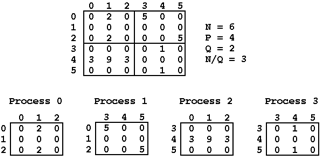
\includegraphics[width=0.8\textwidth]{matrix_foxImage.png}
  \caption{Speedup of the Fox algorithm for different matrix sizes.}
  \label{fig:speedup}
\end{figure}

\section{Implementation}
\subsection{Data Structures}
They were defined two main data types:
\begin{itemize}
  \item \textbf{GRID\_INFO\_TYPE:} Structure that stores the topology of MPI processes (grid, communicators by row and column, dimensions, and identifiers of each process);
  \item \textbf{LOCAL\_MATRIX\_TYPE:} Structure that represents a local block of the matrix, with size \(n_b = N/Q\) and a pointer to the dynamically allocated data.
\end{itemize}

Each process maintains local copies of three matrices: \texttt{A\_local}, \texttt{B\_local} and \texttt{C\_local}. The infinite value is represented by \texttt{INT\_MAX = $10^9$}, and the diagonal is forced to zero.

\subsection{Data Distribution}
The input matrix is read only by process 0, which splits it into blocks of size \((n_b \times n_b)\) and distributes them to the remaining processes using \texttt{MPI\_Send} and \texttt{MPI\_Recv}. This process implements a 2D block distribution, ensuring that each process has the corresponding sub-block of the original matrix.

\subsection{Communication and Synchronization}
The function \texttt{Setup\_grid()} creates the process grid with \texttt{MPI\_Cart\_create}, as well as specific communicators for rows and columns. In the \texttt{Fox()} function, each iteration executes:
\begin{enumerate}
  \item Block diffusion of \(A\) along the row with \texttt{MPI\_Bcast};
  \item Local min-plus multiplication between blocks of \(A\) and \(B\);
  \item Update of the local block \(C\) with the minimum between the current value and the new;
  \item Rotation of the blocks of \(B\) using \texttt{MPI\_Sendrecv\_replace()}.
\end{enumerate}

\subsection{Repeated Squaring and Convergence}
Multiplication is repeated \(\lceil \log_{2} N \rceil\) times. In each iteration, \texttt{Fox()} is called with the same input blocks (\(A=B\)), and the result is swapped between the variables \texttt{src} and \texttt{dst}. The program terminates when the iterations are completed, producing the final result in \texttt{src}.

\subsection{Input and Output}
Process 0 reads the array from \texttt{stdin}, substituting 0 and -1 with \texttt{INT\_MAX}. After the iterations, the result blocks are gathered with \texttt{MPI\_Recv} and \texttt{MPI\_Send} back to process 0, which prints the final matrix. Entries without a path are returned as \(-1\).

\section{Results and Evaluation}



\section{Partial Conclusions}
The program implements the foundations of the min-plus product and Fox's algorithm in MPI, combined to solve the APSP via \emph{Repeated Squaring}.

\begin{thebibliography}{9}
\bibitem{cormen2009introduction}
Cormen, T. H., Leiserson, C. E., Rivest, R. L., \& Stein, C. (2009).
\textit{Introduction to Algorithms} (3rd ed.).
MIT Press.

\bibitem{fox1987}
Fox, G. C., Otto, S. W., \& Hey, A. J. (1987).
\textit{Matrix algorithms on a hypercube I: Matrix multiplication}.
Parallel Computing, 4(1), 17–31.

\bibitem{pacheco1998}
Pacheco, P. S. (1998).
\textit{A User's Guide to MPI}.
San Francisco: Department of Mathematics, University of San Francisco.

\end{thebibliography}


\vspace{0.3cm}
\textit{Note: The complete source code (\texttt{cp\_projecti.c}) is attached in the ZIP file submitted along with this report.}


\end{document}